
%% MAB_for_task_allocation.tex
%% V1.4a
%% 2016/04/15
%% by lemondy
%%
%% This is a skeleton file demonstrating the use of IEEEtran.cls
%% (requires IEEEtran.cls version 1.8a or later) with an IEEE
%% Computer Society journal paper.
%%

\documentclass[10pt,journal,compsoc]{IEEEtran}
%

\usepackage{graphicx}
\usepackage{amsmath}
\usepackage{epsfig}
\usepackage{latexsym}
\usepackage{amsfonts}
\usepackage{amssymb}
\usepackage[noend]{algorithmic}
\usepackage[ruled]{algorithm}
\usepackage{paralist}
\usepackage{caption}
\usepackage{multirow}
\usepackage{amsthm}

\newtheorem{Lemma}{Lemma}
\newtheorem{definition}{Definition}
\newtheorem{Theorem}{Theorem}

%����
\usepackage{indentfirst}
%
\usepackage{booktabs}

\newtheorem{myDef}{Definition}
\newtheorem{myTheo}{Theorem}
%����
\usepackage[no-math]{xeCJK}
\setCJKmainfont[BoldFont=SimHei, ItalicFont=KaiTi]{SimSun}
\setCJKmonofont{KaiTi}


% *** CITATION PACKAGES ***
%
\ifCLASSOPTIONcompsoc
  % IEEE Computer Society needs nocompress option
  % requires cite.sty v4.0 or later (November 2003)
  \usepackage[nocompress]{cite}
\else
  % normal IEEE
  \usepackage{cite}
\fi




% *** GRAPHICS RELATED PACKAGES ***
%
\ifCLASSINFOpdf
  % \usepackage[pdftex]{graphicx}
  % declare the path(s) where your graphic files are
  % \graphicspath{{../pdf/}{../jpeg/}}
  % and their extensions so you won't have to specify these with
  % every instance of \includegraphics
  % \DeclareGraphicsExtensions{.pdf,.jpeg,.png}
\else
  % or other class option (dvipsone, dvipdf, if not using dvips). graphicx
  % will default to the driver specified in the system graphics.cfg if no
  % driver is specified.
  % \usepackage[dvips]{graphicx}
  % declare the path(s) where your graphic files are
  % \graphicspath{{../eps/}}
  % and their extensions so you won't have to specify these with
  % every instance of \includegraphics
  % \DeclareGraphicsExtensions{.eps}
\fi




%\ifCLASSOPTIONcaptionsoff
%  \usepackage[nomarkers]{endfloat}
% \let\MYoriglatexcaption\caption
% \renewcommand{\caption}[2][\relax]{\MYoriglatexcaption[#2]{#2}}
%\fi



% correct bad hyphenation here
\hyphenation{op-tical net-works semi-conduc-tor}


\begin{document}
%
% paper title
% Titles are generally capitalized except for words such as a, an, and, as,
% at, but, by, for, in, nor, of, on, or, the, to and up, which are usually
% not capitalized unless they are the first or last word of the title.
% Linebreaks \\ can be used within to get better formatting as desired.
% Do not put math or special symbols in the title.
\title{A Multiarmed Bandit Incentive Mechanism for\\ Task Allocation in Crowdsensing}
%

\author{Michael~Shell,~\IEEEmembership{Member,~IEEE,}
        John~Doe,~\IEEEmembership{Fellow,~OSA,}
        and~Jane~Doe,~\IEEEmembership{Life~Fellow,~IEEE}% <-this % stops a space
\IEEEcompsocitemizethanks{\IEEEcompsocthanksitem M. Shell is with the Department
of Electrical and Computer Engineering, Georgia Institute of Technology, Atlanta,
GA, 30332.\protect\\
% note need leading \protect in front of \\ to get a newline within \thanks as
% \\ is fragile and will error, could use \hfil\break instead.
E-mail: see http://www.michaelshell.org/contact.html
\IEEEcompsocthanksitem J. Doe and J. Doe are with Anonymous University.}% <-this % stops an unwanted space
\thanks{Manuscript received April 19, 2005; revised September 17, 2014.}}



% The paper headers
\markboth{Journal of \LaTeX\ Class Files,~Vol.~13, No.~9, September~2014}%
{Shell \MakeLowercase{\textit{et al.}}: Bare Demo of IEEEtran.cls for Computer Society Journals}

\IEEEtitleabstractindextext{%
\begin{abstract}
The multi-armed bandit problem has attracted remarkable attention in the machine learning community and many efficient algorithms have been proposed to handle the so-called exploitation-exploration dilemma in various bandit setups. At the same time, significantly less effort has been devoted to adapting bandit algorithms to particular architectures, such as sensor networks, multi-core machines, or peer-to-peer (P2P) environments, which could potentially speed up their convergence.
\end{abstract}

% Note that keywords are not normally used for peerreview papers.
\begin{IEEEkeywords}
Task Allocation, multiarmed bandits, cellular network, reward maximization, Thompson sampling
\end{IEEEkeywords}}


% make the title area
\maketitle

\IEEEdisplaynontitleabstractindextext
% \IEEEdisplaynontitleabstractindextext has no effect when using
% compsoc or transmag under a non-conference mode.



% For peer review papers, you can put extra information on the cover
% page as needed:
% \ifCLASSOPTIONpeerreview
% \begin{center} \bfseries EDICS Category: 3-BBND \end{center}
% \fi
%
% For peerreview papers, this IEEEtran command inserts a page break and
% creates the second title. It will be ignored for other modes.
\IEEEpeerreviewmaketitle



\IEEEraisesectionheading{\section{Introduction}\label{sec:introduction}}


Mobile crowdsensing is a new type of collaboration which involves a crowd of mobile users who uses their carried smart phone to execute some complex computation or sensing services in some environment. Since it can utilize the mobility of users to solve large-scale mobile sensing tasks, it has stimulated a number of attractive applications, such as urban WiFi characterization, traffic information mapping, and so on. Moreover, there have been some platforms, frameworks, and incentive mechanism, designed for crowdsensing in all kinds of scenario.\cite{xiao2015multi}\cite{jain2014multiarmed}

Consider that a user carried mobile phone in an mobile social network has some independent sensing tasks, such as sample WiFi fingerprint, traffic information mapping, and so on. However, these tasks cost too much time and exceed its processing ability. Then, it requests other mobile users for help by starting a crowdsensing. In this scenario, the requester will send tasks to and receive results from other mobile users, of which can by calling other or by send message to communicate. And it often involves large size data transmissions, however, we can incent many users joining it, such that can decrease every user's work time. \cite{xiao2015multi} adapts short-distance wireless communication technologies (e.g., WiFi or Bluetooth), in contrast, we consider a different communication technology, which through cellular network get in touch with each other. In this situation, the requester doesn't have to stay not far from the worker, and what's more, the requester can do another work after publishes tasks. Fig.1 depicts a simple example of a task allocation procedure in crowdsensing. At some time, the requester wants to collect some data, and then it send message to the work ask they bid for the task. After the work return their bid and workload, then the requester make a decision to choose a best worker to handle these tasks. The best worker means he will finish the worker very well and at the same time the bid is reasonable. Then, an important problem is how the requester allocates these task to workers, so as to for every task can choose a best worker to finish it.

%\begin{figure}[!t]
%  \centerline{
%  \begin{tabular}{cc}
%  \epsfysize=4in\epsfbox{./fig/mobile_social_network.eps}
%  \end{tabular}}
%  \caption{Results on random networks ($n=20$, $m=10$). }
%  \label{fig:k_throwboxes_random_20}
%\end{figure}
\begin{figure}[H]
\begin{center}
  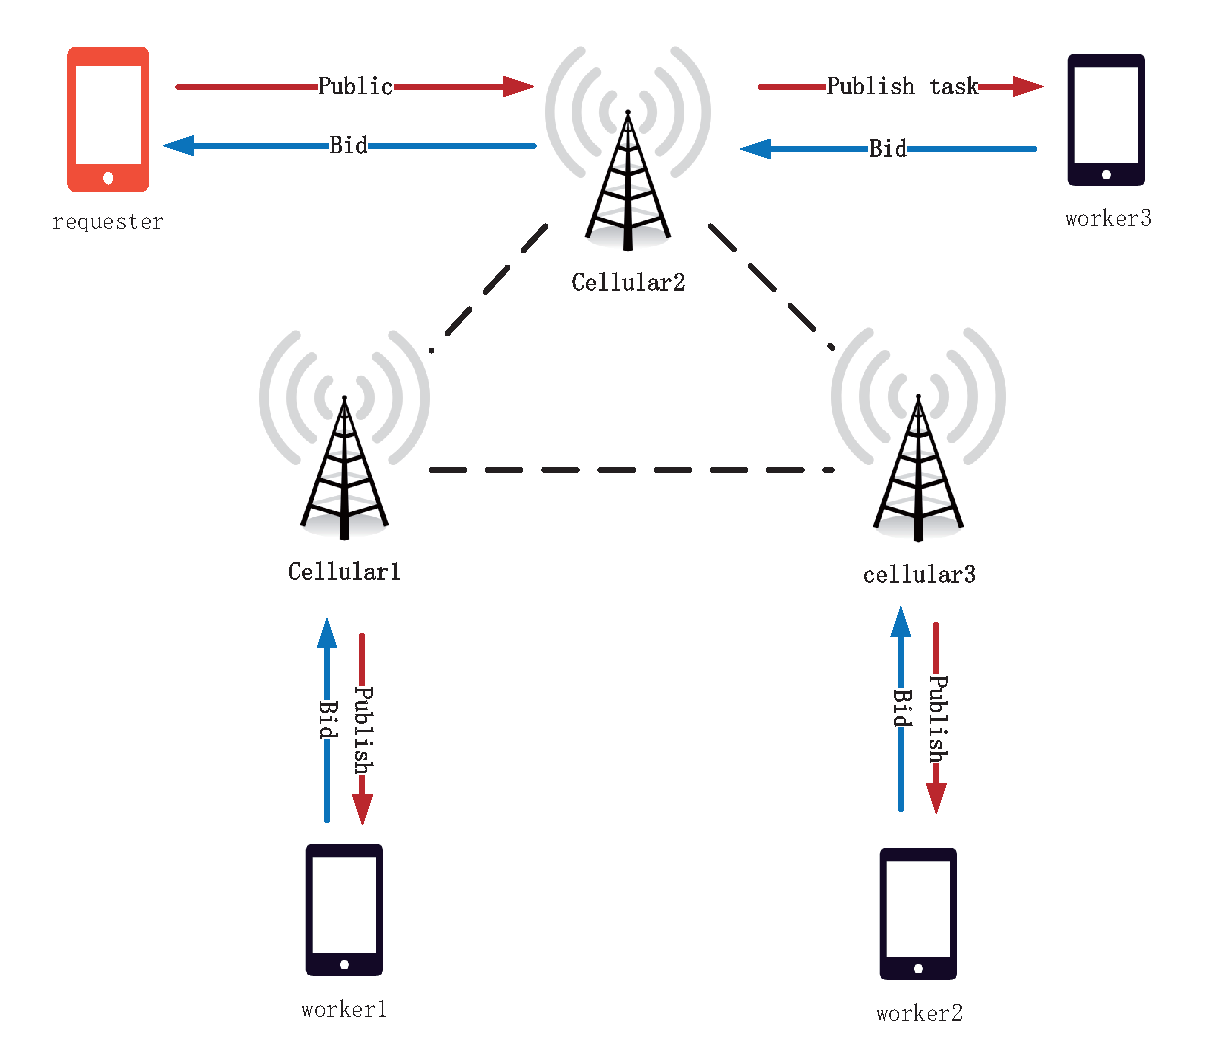
\includegraphics[width=0.4\textwidth]{./fig/mobile_crowdsensing.eps}
  \caption{mobile social network}\label{MSN}
\end{center}
\end{figure}

In this paper, we focus on the above task allocation problem. In this problem, choosing a best worker from the requester's contacts. Selects best worker just like choose excellent contractor, which will let the utility maximize of the requester.

To solve the above task allocation problem in mobile crowdsensing, we proposed a based multi-armed bandits algorithm with incentive mechanism, which is called Thompson sampling task allocation(TS-TA). We choose Thompson sampling to handle this problem.

Thompson sampling(TS) is one of the earliest heuristics for multi-armed bandit problems. The first Bayesian heuristics is around 80 years old, dating to Thompson(1933). Since then, it has been rediscovered numerous times independently in the context of reinforcement learning, e.g., in [?][?]. It is a member of the family of \textit{randomized probability matching} algorithms. The basic idea is to assume a simple prior distribution on the underlying parameters of the reward distribution of every arm, and at every time step, play an arm according to its posterior probability of being the best arm. The general structure of TS for the contextual bandits problem involves the following elements:

 \begin{itemize}
   \item a set $\theta $ of parameters ${\tilde \mu }$ ;
   \item a prior distribution $P({\tilde \mu})$ on these parameters;
   \item past observations $D$ consisting of (context b, reward r) for the past time steps
   \item a likelihood function $P(r|b,\tilde \mu )$, which gives the probability of reward given a context b and a parameter ${\tilde \mu}$;
   \item a posterior distribution $P(\tilde \mu |D) \propto P(D|\tilde \mu )P(\tilde \mu )$, where $P(D|\tilde \mu)$  is the likelihood function.
 \end{itemize}

 In each round, TS plays an arm according to its posterior probability of having the best parameter. A simple way to achieve this is to produce a sample of parameter for each arm, using the posterior distribution, and play the arm that produces the best sample. More specifically, the following are our major contributions in this paper:
 \begin{enumerate}
   \item We formulate the problem into a linear payoffs MAB problem that shall find optimal worker when there are tasks need to be allocated. Then we proposed a novel algorithm, Thompson Sampling Task Allocation(TS-TA) which make sure the worker is truthful and rational.
   \item We proved that the regret has a lower bound, where any MAB algorithm has to suffer.
   \item We conduct our simulations on real traces dataset to evaluate the TS-TA algorithm. The results show that the proposed algorithm can achieve O(logT) lower bound.
 \end{enumerate}
The remainder of the paper is organized as follows.We present a summary of the relevant work in Section 2. In Section 3, we introduce how multi-armed bandits can be model for task allocation problem. In Section 4, we formulate the task allocation problem. And next in Section 5, we proposed our algorithm thompson sampling for task allocation, which according to the thompson sampling to choose a worker to finish current work and then decide to give how much payment to that worker. In Section 6, we do some theory work to prove our algorithm's regret is bounded. In Section 8, we provide a simulation on a real dataset to  verify our algorithm. Conclusions is provided in Section 9.
\section{RELATED WORK}

\subsection{Task allocation}
In this paper, we focus on the task assignment problem in mobile crowdsensing, which involves a lot of mobile users in solving a large job through their carried mobile devices \cite{ganti2011mobile}. By far, there have been several frameworks, platforms, and incentive mechanisms designed for crowdsensing system, \cite{cardone2013fostering}, \cite{farshad2014urban},\cite{feng2014trac},\cite{he2014toward}, \cite{ganti2011mobile}. Among them, the most related work is the LRBA algorithm designed for a task allocation problem in mobile crowdsensing \cite{he2014toward}. Unlike our work, the problem in this work pay attention to how to choose the worker who will provide better service and the tasks are location dependent.

On the other hand, our task assignment problem is also different from traditional parallel machine scheduling problems. In fact, there have been thousands of papers on parallel machine scheduling problems by far. Literatures \cite{allahverdi2008survey},\cite{cheng1990state} have made a detail review on these works. Even in recent years, there is still much research on the complex parallel machine scheduling problems, such as \cite{alidaee2014parallel},\cite{chekuri2001approximation}. The most related works among the existing researches is \cite{liu2015online}, who consider a crowd-sourcing problem where in the process of labeling massive datasets, multiple labelers with unknown annotation quality must be selected to perform the labeling task for each incoming data task. And they formulate it to MAB problems, then proposed an algorithm to solve it. In contrast, the tasks allocates has to consider the current context and then select a worker, what's more, the payment of workers' efforts also be taken into consideration. More specifically, each task being sent to a mobile worker is according to thompson sampling algorithm and the payment is decided just like an auction mechanism just like what have existed in crowdsourcing. Such a unique task assignment model makes our problem different from existing parallel machine scheduling problems.


\subsection{MAB Algorithms}
The fundamental challenge in bandit problems is the the need for balancing exploration and exploitation. Changing the aim of maximize reward to minimize the regret multiple experiments, an algorithm A will exploits its past experience to select the arm that appears best. On the other hand, this seemingly optimal arm may in fact be suboptimal, due to imprecision in A's knowledge. In other to avoid this undesired situation, A has to explore by actually choosing seemingly suboptimal arms to gather more information about them. Exploration can increasing short-term regret since some suboptimal arms may be chosen. However, obtaining information about the arms' average payoffs can refine A's estimate of the arms' payoffs and in turn reduce long-term regret. Clearly, neither a purely exploring nor a purely exploiting algorithm works best in general, and a good tradeoff is needed.

There are a lot of literatures available on the MAB problem. Our problem belongs to the stochastic MAB setting, where the distribution function of reward of each arm is known but the parameter is unknown. A recent survey by Bubeck and Cesa-Bianchi \cite{bubeck2012regret} compiles several variations on stochastic and non-stochastic MAB problems. Our setting is very close to \cite{agrawal2012thompson} where a general bandit problem with linear payoff function which is related to the context. Our setting is a further concretization, as the context in our algorithm is concrete and we do some experiments to decide the weights of different feature which are used for the context.


\begin{table}[!t]
%% increase table row spacing, adjust to taste
\renewcommand{\arraystretch}{1.3}

\centering
%% Some packages, such as MDW tools, offer better commands for making tables
%% than the plain LaTeX2e tabular which is used here.
\begin{tabular}{|c|c|}
\hline
\hline
Multi-armed Bandit(MAB) & Task Allocation(TA)\\
\hline
\hline
Player & Requester\\

Armed bandit & Workers\\

Pull level & Select worker\\
\hline
\hline
\end{tabular}
\caption{Parallel between Multi-armed bandit and Task Allocation}
\end{table}


\begin{table}[!t]
%% increase table row spacing, adjust to taste
\renewcommand{\arraystretch}{1.3}
\centering
\begin{tabular}{|c|c|}
\hline
\hline
Notation & Description\\
\hline
\hline
K & Set of all workers in the requester's contacts\\

m & Number of tasks\\

$b _i(t)$ & Context of arm i at time t\\

$\mu$ & The prior parameter of the arm\\

$r _i(t)$ & The reward of arm i at time t\\

$\pi$ & The allocation mechanism\\

$RE ^ \pi$ & The total regret\\

${p _i}^t$ & Payment of arm i\\
\hline
\hline
\end{tabular}
\caption{Notation used}
\end{table}


% Note that the IEEE does not put floats in the very first column
% - or typically anywhere on the first page for that matter. Also,
% in-text middle ("here") positioning is typically not used, but it
% is allowed and encouraged for Computer Society conferences (but
% not Computer Society journals). Most IEEE journals/conferences use
% top floats exclusively.
% Note that, LaTeX2e, unlike IEEE journals/conferences, places
% footnotes above bottom floats. This can be corrected via the
% \fnbelowfloat command of the stfloats package.
\section{A Parallel with Crowdsourcing}
"Crowdsourcing is the act of taking job traditionally performed by a designated agent(usually an employee) and outsourcing it to an undefined, generally large group of people in the form of an open call", this is what Jeff Howe ever offered the definition of crowdsourcing. The designated agent is often called the requester, while people working on the task are called crowd workers. The requester needs to assign the task to these workers with unknown capability and willingness to complete the task based on the goals to achieve. In mobile crowdsensing network, there is a task publisher at some time, and he/she can chooses a worker from his/her contacts. The task publisher just like the requester, while his/her contacts just like the group of works. Table 1 precisely demonstrates this paralle between crowdsoucing and mobile crowdsensing.

\section{A Parallel with MAB}


\section{Model\&Problem}
%Transform the task allocation into a multi-armed bandit problem.

\subsection{Model for Task Allocation}
Consider a network denoted by a graph ${G^t} = ({V^t},{E^t})$ at time t with a set ${V^t} = \{ {v_i}|i = 1,...,K\}$ of K nodes represented the node set who meet the task requester node represented by ${v_0}$ at time t, a set E of edges denoting ${v_0}$ can communicate with other nodes. And the graph is star network structure. The system is been divided into time slot, and at each round t, node ${v_0}$ has K choices of relay node, where relay nodes are i.i.d. Suppose the ability of every node accomplish a task as stochastic process ${\chi _i}(t)$ over time with a mean ${\mu _i} \in [0,1]$, as done in many previous works [1] [2] [3].

\setlength{\parindent}{2em}At each round t, an K-dimensional \emph{strategy} vector ${\Phi _0}(t) = \{ {\Phi _{0,i}}|i = 1,...,K\}$ is selected under some \emph{policy} from the \emph{feasible strategy set} F. Here ${\Phi _{0,i}}$ is the index of relay node selected by node carried message in strategy $\Phi _0$. We use i=1,...,K to index strategies of feasible set F in XXXXX. By feasible we mean at that time slot, carried message node meet another k nodes(who can communicate with the message carrier directly). When a strategy $\Phi _0$ is determined, then one node $v _i$ will be selected, and it will give back a reward $r _i(t)$. And then the total reward of T round is defined as $R = \sum\nolimits_{t = 1}^T {r(t)}$. The goal of this allocation problem is to maximize the accumulated reward $R$ over the T rounds. Obviously, if the reward of every node is constant, then we can simply choose the node who will have maximize reward every time slot. While in our problem, the reward is variable over time. And it's probability distribution follows $f(x,\theta )$ where $\theta$ is an unknown parameter. The gap between the actual total reward we get and the optimal total reward theoretically is call regret of the algorithm, and it can be formally written as $RE = \sum\nolimits_{t = 1}^T {{r^*}(t)}  - \sum\nolimits_{t = 1}^T {r(t)}$, where $r^*$ is the max reward we can get every time slot. The goal of the algorithm is to keep the regret $RE$ as low as possible.

\setlength{\parindent}{2em}An allocation strategy(also called a policy) $\pi$ specifies the action chosen by the task requester(carried message node) at each time in the system. Formally, $\pi$ is a sequence of random variables $\pi  = \{ {\pi ^1},{\pi ^2},...,{\pi ^T}\}$ where ${\pi ^t} = \{ a_1^t,a_2^t,...,a_k^t\}$ is the vector of zeros and ones(deterministic mechanism). If $a_i^t=1$ then node i will be chosen as a relay node at slot t, whereas, $a_i^t=0$ means node i doesn't be chosen at all, i.e., $\forall t,\sum\nolimits_i {{a^t}}  \le 1$.

%%����arm��payoff�����Եġ�
There are K arms at time t for a requester, a context vector ${b_i}(t) \in {R^d}$, is revealed for every arm i. These context vectors are chosen by a requester in an adaptive manner after observing the arms played and their rewards up to time t-1, i.e. history $H_{t-1}$,

${H_{t - 1}} = \{ a(\tau ),{r_{a(\tau )}}(\tau ),{b_i}(\tau ),i = 1,...,K,\tau  = 1,...,t - 1\} $,

where $a(\tau)$ denotes the worker played at time $\tau$, ${r_{a(\tau )}}(\tau )$ denotes when chose arm $a$ the reward you have gotten. Given ${b_i}(t)$, the reward for arm i at time t is generated from an (unknown) distribution with mean ${b_i}(t)\mu$, where $\mu \in {R^d}$ is a fixed but unknown parameter \cite{agrawal2012thompson}.

$E[{r_i}(t)|\{ {b_i}(t)\} _{i = 1}^K,{H_{t - 1}}] = E[{r_i}(t)|\{ {b_i}(t)\} ] = {b_i}{(t)^T}\mu$.

At every time slot t, for the contextual bandit problem algorithm needs to select an arm $a(t)$ to play, using history $H _t-1$ and current contexts ${b _i}(t), i=1,...,K$. Let ${a^*}(t)$ denote the optimal arm at time t, i.e. ${a^*}(t) = \arg {\max _i}{b_i}{(t)^T}\mu $. And then the regret of strategy $\pi$ at time t is defined as follows:

\begin{equation}
{RE^\pi } = \sum\limits_{t = 1}^T {\{ {r^*}(t) - \sum\limits_{i = 1}^K {{a_i}{r_i}(t)} \} }
\end{equation}

The objective is to minimize the total regret $RE$ in overall T. The time horizon T is finite but possibly unknown.

Suppose that ${\eta _{i,t}} = {r_i}(t) - {b_i}{(t)^T}\mu $ is conditionally R-sub-Gaussian for a constant $c \ge 0$ just like in agrawal2012thompson, i.e.,

${\forall \lambda  \in R}$,$E[{e^{\lambda {\eta _{i,t}}}}|\{ {b_i}(t)\} _{i =1}^N,{H_{t - 1}}] \le \exp (\frac{{{\lambda ^2}{c^2}}}{2})$

This assumption is satisfied whenever ${r_i}(t) \in [{b_i}{(t)^T}\mu  - c,{b_i}{(t)^T}\mu  + c]$ (see Remark 1 in Appendix Filippi et al.(2010)). We will also assume that $\left\| {{b_i}(t)} \right\| \le 1,\left\| \mu  \right\| \le 1$, and $regre{t_i}(t) \le 1$ for all i,t (the norms, unless otherwise indicated, are $L _2$-norms). These assumptions are required to make the regret bounds scale-free, and are standard in the literature on this problem. If $\left\| {{b_i}(t)} \right\| \le \alpha ,\left\| \mu  \right\| \le \alpha , regret_i (t) \le \alpha$ instead, then our regret bounds would increase by a factor of $\alpha$.


we now define some of the desirable properties that an allocation policy show satisfy:\\
\emph{\textbf{Definition 1} Allocation Efficiency(AE)}: An allocation policy $\pi$ is said to be allocation efficiency if it minimize the regret. Formally, $\pi$ is allocation efficiency if:

\setlength{\parindent}{6em}$\pi  = \mathop {\arg \min R{E^\pi }}\limits_\pi$\\

\setlength{\parindent}{0em}\emph{\textbf{Definition 2} Dominant Strategy Incentive Compatibility(DSIC):} Mechanism $M$ is said to be DSIC if truth telling is a dominant strategy for all the workers. Formally,\\

\emph{\textbf{Definition 3} Individual Rationality(IR):} Mechanism M is said to be IR for a worker if participating in mechanism always gives him positive utility. Formally,
%table
%\begin{tabular}{c|c}
%\toprule
%title&meaning\\
%\hline
%a&variable\\
%b&cdedfda\\
%c&kkkkkk\\
%\bottomrule
%\end{tabular}


\subsection{Problem}\setlength{\parindent}{2em}
Consider a mobile crowdsensing in the mobile social network. Without loss of generality, we let the requester be user ${v_0}$, and suppose that the requester has $m$ homogeneous mobile sensing tasks in one cycle, denoted by $j(n)$. The length of one cycle is $T$, and these tasks might be different types of task in different cycle. For simplicity, we assume that every requester will choose one worker from who ever get contacted with the requester for every task allocation and the requester's contact is built at the beginning within time $t$. It means if someone get contact with the requester during the period of the beginning $t$, the one will be add to the requester's contacts, regardless of who is the caller.

In this paper, we focus on how to choose a sequence of workers so as to maximize the utility of requester in every cycle.


\section{Task allocation algorithm}

\subsection {Thompson Sampling for Task Allocation}
\setlength{\parindent}{2em}In this section, we will explain our Thompson Sampling algorithm for task allocation with incentive mechanism. The most important challenge is to balance exploitation with exploration. That is, we have two somewhat conflicting goals: (a) quickly find the best arm to pull and (b) pull the best arm as often as possible. Now we'll introduce the asymptotic optimal algorithm: Thompson Sampling.

Before I introduce the Thompson sampling, let's build up some intuition. If we have an infinite amount of pulls, then we know exactly what the expected rewards are, and there is no reason to ever explore. When we have a finite number of pulls, then we have to explore and the reason is that we are uncertain of what is the best arm. The right machinery to quantify uncertainty is the probability distribution. In Bayesian thinking, we want to use the entire probability distribution. Let's define ${p_a}(r)$ is the probability distribution from which rewards are drawn. That's what controls the bandit. We don't need to estimate the entire distribution for infinite amount of pulls, because all we care about is its mean ${\mu _a}$. What we will do is encode our uncertainty of ${\mu _a}$ in the probability distribution $p({\mu _a}|dat{a_a})$, and then use that probability distribution to decide when to explore and when to exploit.

let's say more clearly about the two probability:\\
 ${p_a}(r)$ - the probability distribution that bandit $a$ uses to generate rewards when it is pulled.\\
 $p({\mu _a}|dat{a_a})$ - the probability distribution of where we think the mean of ${p_a}(r)$ after observing some data.\\

 With Thompson sampling you keep around a probability distribution $p({\mu _a}|dat{a_a})$ that encodes your belief about where the expected reward ${\mu _a}$ is for arm $a$. For the simple coin-flip case, we can use the convenient Beta-Bernoulli model, and the distribution at round t after seeing ${S _a,t}$ successes and ${F _a,t}$ failures for arm $a$ is simply:\\
 $p({\mu _a}|dat{a_a}) = Beta({S _a,t}+1, {F_a,t}+1)$,\\
 where the added 1's are convenient priors.

 In our problem, we use Gaussian likelihood function and Gaussian prior to design our version of Thompson Sampling algorithm. More precisely, suppose that the likelihood of reward ${r _i}(t)$ at time t, given context ${b _i}(t)$ and parameter ${\mu}$, were given by the pdf of Gaussian distribution $N({b_i}{(t)^T}\mu ,{v ^2})$. Here, $v = R\sqrt {\frac{{24}}{\varepsilon }d\ln (\frac{1}{\delta })} $, with $\varepsilon  \in (0,1)$ which parameterizes our algorithm,just like \cite{agrawal2012thompson}. Let\\

 \setlength{\parindent}{4em}$B(t) = {I_d} + \sum\nolimits_{\tau  = 1}^{t - 1} {{b_{a(t)}}(\tau ){b_{a(t)}}{{(\tau )}^T}} $\\

 \setlength{\parindent}{4em}$\hat \mu (t) = B{(t)^{ - 1}}(\sum\nolimits_{\tau  = 1}^{t - 1} {{b_{a(t)}}(\tau ){r_{a(t)}}(\tau )} )$\\
 Then, if the prior for $\mu$ at time t is given by $N(\hat \mu (t),{v^2}B{(t)^{ - 1}})$, it is easy to compute the posterior distribution at time t+1,\\

 \setlength{\parindent}{4em} $\Pr (\hat \mu |{r_i}(t)) \propto \Pr ({r_i}(t)|\hat \mu )\Pr (\hat \mu)$\\
 as $N(\hat \mu (t),{v^2}B{(t)^{ - 1}})$ (detail of this computation are in Appendix A.1). In our Thompson Sampling algorithm, at every time step t, we will simply generate a sample ${\hat \mu(t)}$ from $N(\hat \mu (t),{v^2}B{(t)^{ - 1}})$, and play the arm $i$ that maximizes ${b_i}{(t)^T}\hat \mu (t)$.

\begin{algorithm}
\caption{TS-TA}
\begin{algorithmic}[3]

\STATE Set $B=I _d, \hat \mu=0_d, f = 0_d$
\FOR {$t=1,2,...,$}
\STATE Sample ${\hat \mu(t)}$ from distribution $N(\hat \mu (t),{v^2}B{(t)^{ - 1}})$.
\STATE Play arm $a(t):=argmax_i{b_i(t)^T\hat\mu(t)}$, and observe reward $r_t$.
\STATE Update $B=B+{b_{a(t)}}(t){b_{a(t)}}{(t)^T}, f=f+ {b_{a(t)}}(t)r_t, \hat \mu (t)=B^{-1} f$.
\IF {${r_t}=1$}
\STATE current arm is i(t), then we need to give him payback.
\STATE choose arm $j(t): = \mathop {\arg \max {\theta _j}(t)}\limits_{j \in K\backslash i}$ and observe reward ${r_t}^\prime $
\STATE Perform a Bernoulli trial with success probability ${{\tilde r}_t}^\prime$ and observe output ${r_t}^\prime$
\IF {${r_t}^\prime =1$}
\STATE ${p_i}^t = min({p_j}^t, p_max)$
\ELSE
\STATE ${p_i}^t=min({p_i}^t,p_max)$
\ENDIF
\ELSE
\STATE do not allocation this task at this round.
\ENDIF
\ENDFOR
\end{algorithmic}
\end{algorithm}

At every step t of Thompson Sampling task allocation algorithm consists of generating a d-dimensional sample ${\tilde \mu }$ from a multi-variate Gaussian distribution, and solving the problem $argmax_i{b_i(t)^T\hat\mu(t)}$. Therefore, even if the number of arms N is large (or infinite), the above algorithm is efficient as long as the problem $argmax_i{b_i(t)^T\hat\mu(t)}$ is efficiently solvable. After choose an arm, then, we should decide to give how much payment to that work. For this part, we have to make sure the worker is rational and truthful. For the payment, we first record the worker's bid who have the max ${b_i(t)^T\hat\mu(t)}$, and then we temporarily put the worker aside who has been selected just now, and selected the other worker who has the max ${b_i(t)^T\hat\mu(t)}$ over the rest of workers. The requester then collects the rest worker's bid and choose a property one's bid, which will be as the payment of the first worker. Just as in our algorithms.

\section{Analysis of AT-algorithm}
\setlength{\parindent}{2em}In this section, we provide theoretical guarantees for TS-TA. The contextual version of the multi-armed bandit problem presents new challenges for the analysis of TS algorithm, and the techniques used so far for analyzing the basic multi-armed bandit problem by \cite{agrawal2011analysis} do not seem directly applicable.

%use label, you can in other place reference this theory through \ref{IR}
\begin{Theorem}\label{IR}
TS-TA is IR for all worker.
\end{Theorem}

\begin{proof}[Proof of TS-TA is IR]
Here is the proof of IR.
\end{proof}

\begin{Theorem}\label{DSIC}
TS-TA is DSIC.
\end{Theorem}

\begin{proof}
here is proof of DSIC.
\end{proof}

\begin{Lemma}
our regret is bounded.
\end{Lemma}



\section{Simulation Experiments}
\setlength{\parindent}{2em}This subsection gives a detail description of our experimental setup, including data collection, feature construction, performance evaluation.

\subsection{Data Collection}
Our dataset comes from MIT Reality Mining. It collected from 100 mobile phone users over the course of 9 month (September 2004 to June 2005) at MIT. The dataset includes the participants' message and phone call history, Bluetooth discovery records, answers of a survey etc. We again extract communication information and location based on phone call history. We use the before six month data as training set and the later part is used for testing algorithm. In train, we statistic every user who ever have gotten in touch with him, including call and message history. Through this, we can confirm everyone's contacts, and then in our algorithm we will regard the k members of his contacts as k arm bandits.

\subsection{Feature Construction}

We now describe the feature(also called context) constructed for our experiments. The features are used for our reward model, for we have define the reward as a linear payoffs.
Context means what situation the requester meets in order to allocate the works, for example, how much is the worker's bid for the task, how many size there spares in worker's buffer and so on. Because when meets different context, the requester's choice is different. We start with raw context that were selected by "support". The support of a feature is the fraction of context. To reduce noise in the data, we only selected features with high support and do some preprocess. Then, each worker was originally represented by a raw feature vector, which include: \begin{itemize}
                                                      \item \textbf{worker's bid for concurrent task}: the requester also should think of its utility (task's value minus the payment), and want to maximize its own utility.
                                                      \item \textbf{worker's buffer size}: every worker have limits space or ability to finish limited worker, for which will make sure it suitable for reality.
                                                      \item \textbf{the probability of accomplish a task}: this relates to worker's location and it's ability or willing to finish the task;
                                                      \item \textbf{the number of have accomplished a kind of task}: there will exits several kinds of task, we will record the worker have finished how many times for every kind of task.
                                                      \item \textbf{centrality}: this will be viewed as a factor, which may affect the requester's decision.
                                                    \end{itemize}
For this feature, we will do the normalization to make the feature's value belong to [0,1]. Other than these features, no other information was used to identify context.
\subsection{Performance}
This section we will show the result of experiments.
\section{Conclusion}

\setlength{\parindent}{2em}In this paper, we study the task allocation problem for crowdsensing. In order to select the best worker from the requester's contacts, we proposed thompson sampling allocation algorithm with incentive mechanism. This algorithm can make sure long run and keep the regret stay low. We showed that intuition from crowdsourcing mechansim is useful, and our algorithm follow the DISC and IR constrains. Analysis of TS-TA showed that it achieves regret of .




% if have a single appendix:
%\appendix[Proof of the Zonklar Equations]
% or
%\appendix  % for no appendix heading
% do not use \section anymore after \appendix, only \section*
% is possibly needed

% use appendices with more than one appendix
% then use \section to start each appendix
% you must declare a \section before using any
% \subsection or using \label (\appendices by itself
% starts a section numbered zero.)
%


\appendices
\section{Proof of the First Zonklar Equation}
Appendix one text goes here.

% you can choose not to have a title for an appendix
% if you want by leaving the argument blank
\section{}
Appendix two text goes here.


% use section* for acknowledgment
\ifCLASSOPTIONcompsoc
  % The Computer Society usually uses the plural form
  \section*{Acknowledgments}
\else
  % regular IEEE prefers the singular form
  \section*{Acknowledgment}
\fi


The authors would like to thank...


% Can use something like this to put references on a page
% by themselves when using endfloat and the captionsoff option.
%\ifCLASSOPTIONcaptionsoff
 % \newpage
%\fi



% trigger a \newpage just before the given reference
% number - used to balance the columns on the last page
% adjust value as needed - may need to be readjusted if
% the document is modified later
%\IEEEtriggeratref{8}
% The "triggered" command can be changed if desired:
%\IEEEtriggercmd{\enlargethispage{-5in}}

% references section

% can use a bibliography generated by BibTeX as a .bbl file
% BibTeX documentation can be easily obtained at:
% http://www.ctan.org/tex-archive/biblio/bibtex/contrib/doc/
% The IEEEtran BibTeX style support page is at:
% http://www.michaelshell.org/tex/ieeetran/bibtex/
%\bibliographystyle{IEEEtran}
% argument is your BibTeX string definitions and bibliography database(s)
%\bibliography{IEEEabrv,../bib/paper}
%
% <OR> manually copy in the resultant .bbl file
% set second argument of \begin to the number of references
% (used to reserve space for the reference number labels box)
%\begin{thebibliography}{1}

%\bibitem{IEEEhowto:kopka}
%H.~Kopka and P.~W. Daly, \emph{A Guide to \LaTeX}, 3rd~ed.\hskip 1em plus
%  0.5em minus 0.4em\relax Harlow, England: Addison-Wesley, 1999.

%\end{thebibliography}

%��������

\renewcommand\refname{REFERENCES}
\bibliographystyle{plain}
\bibliography{./myreference}


% biography section
%
% If you have an EPS/PDF photo (graphicx package needed) extra braces are
% needed around the contents of the optional argument to biography to prevent
% the LaTeX parser from getting confused when it sees the complicated
% \includegraphics command within an optional argument. (You could create
% your own custom macro containing the \includegraphics command to make things
% simpler here.)
%\begin{IEEEbiography}[{\includegraphics[width=1in,height=1.25in,clip,keepaspectratio]{mshell}}]{Michael Shell}
% or if you just want to reserve a space for a photo:

%\begin{IEEEbiography}{Michael Shell}
%Biography text here.
%\end{IEEEbiography}

% if you will not have a photo at all:
%\begin{IEEEbiographynophoto}{John Doe}
%Biography text here.
%\end{IEEEbiographynophoto}

% insert where needed to balance the two columns on the last page with
% biographies
%\newpage

%\begin{IEEEbiographynophoto}{Jane Doe}
%Biography text here.
%\end{IEEEbiographynophoto}

% You can push biographies down or up by placing
% a \vfill before or after them. The appropriate
% use of \vfill depends on what kind of text is
% on the last page and whether or not the columns
% are being equalized.

%\vfill

% Can be used to pull up biographies so that the bottom of the last one
% is flush with the other column.
%\enlargethispage{-5in}


% that's all folks
\end{document}


